\documentclass[12pt]{report}
    \usepackage{blindtext}
    \usepackage{hyperref}
    \usepackage{tocloft}
    \usepackage{natbib}
    \usepackage{graphicx}
    % \usepackage[newfloat]{minted}
    \usepackage{caption}
    \usepackage{amsmath}
    \usepackage[table]{xcolor}
    \usepackage[a4paper, total={6in, 8in}]{geometry}
    \newenvironment{longlisting}{\captionsetup{type=listing}}{}
    \title{%
      GPT-2 Based Meme Generator\\~\\
      \large Final Year Project (CTEC3451) \\
        De Montfort University}
    \author{Artem Bobrov (P2547788)}
    \date{Jan 14 2021}
    \setlength{\parindent}{1em}
    \begin{document}
    \maketitle
    \thispagestyle{empty}
    \clearpage
    \tableofcontents
    \setcounter{tocdepth}{1}
    \thispagestyle{empty}
    \clearpage
    \section*{Abstract}
    \addcontentsline{toc}{section}{Abstract}
    
    \paragraph{}
    % Abstract text
    
    This project explores the possibilities of deep learning mechanisms to create and improve the ways of 
    social interaction in the 21st century. The main idea of the project is to prove that modern trained neural networks can 
    synthesise entertainment data based on the input, embedded in an application that is easy to use by every user.
    
    
    \section*{Literature Review}
    \addcontentsline{toc}{section}{Literature Review}
    \paragraph{}

    \subsection*{Introduction}
    \addcontentsline{toc}{subsection}{Introduction}
    \paragraph{}
    
    % Lit review for GPT-2 Backend (Python)

    GPT-2 introduces wide possibilities when it comes to human-like text synthesis. It is developed by OpenAI in February 2019 but the
    release to the public was postponed due to the apprehension that it could potentially be used to conduct malicious and harmful activities. The successor to
    the first GPT family member has been trained on a larger dataset and parameter count with around ten-fold growth. The reason behind
    choosing this exact neural network to produce this project lies in the philosophy followed by its creators. The aim was to take a new approach to the purpose of the system.
    The past neural networks "are better characterized as 'narrow experts' rather than  'competent generalists'" \citep{radford_wu_child_luan_amodei_sutskever_2019} and that was
    the main restraining factor. GPT neural network family uses transformer architecture with attention mechanism which allows faster training due to significantly increased parralelism \citep{attention_is_all_you_need}.
    There are several advantages of using transformer neural networks to process text when compared to convolutional and recurrent neural networks (CNN and RNN). Transformers deal with sentences within a text as a whole and not word by word.
    Self attention is another advantage of transformers since it allows to relate different positions of a single sequence (sentence) to calculate a representation of it \citep{attention_is_all_you_need}.
    And third major difference is positional embeddings. This concept allows the usage of fixed weights that encode information about a specific token in a sequence.
    Convolutional neural networks are very good at processing images and detecting patterns in them. Recurrent neural networks are mainly used in evolutionary robotics to deal with vision \citep{inproceedings}.
    
    
    \clearpage

    \subsection*{Transformer Neural Networks}
    \addcontentsline{toc}{subsection}{Transformer Neural Networks}
    \paragraph{}

    Transformer neural networks continue to gain more popularity among the other artificial intelligence systems for solving 'Natural Language Processing' problems.
    Before transformers gated recurrent units with added attention mechanism were mainly used to process natural language but transformers based on solely that attention mechanism
    has proven that they're more effiecient in solving particular problems \citep{attention_is_all_you_need}. A vast amount of them used encoder-decoder structure in which the encoder maps
    an input sequence of symbol representation to a sequence of continious representation. Using that continious representation the decoder generates an output sequence. Also it uses the
    already generated output as an additional input in order to learn and generate more accurate output.

    Encoder and decoder stacks consist of six identical layers. Every encoder layer has two sub-layers and every decoder layer has three sublayers. The first two sublayers of the decoder are 
    similar to the encoder sublayers. The first is a multi-head self-attention mechanism and the second is a fully connected feed-forward network. The third layer of the decoder works with the output
    of the encoder by performing multi-head attention over it.

    \begin{figure}[htbp]
        \centerline{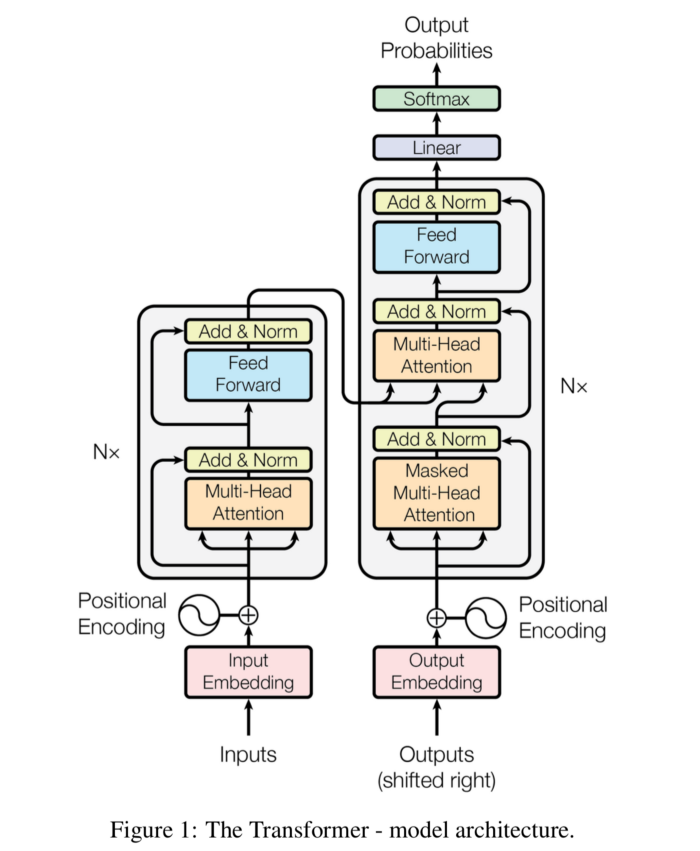
\includegraphics[scale=.35]{img/transformer_model.png}}
        \label{transformer_model}
    \end{figure}

    Since 2019 (release of GPT-2) a lot have changed in the field of transformers and as of November 2020 transformers are separated in different categories which different from each other in some aspects.
    Those categories are: Reformers, Linformers, Linear Transformers, Sinkhorn Transformers, Performers, Synthesizers, Sparse Transformers, and Longformers \citep{LRA_benchmark}. Using this LRA benchmark the
    efficiency of different transformer models could be measured and this could give a better understanding how and in what areas they should be used. This testing suite is available in Python and is open-source so
    everyone could build upon it.

    The suite developers pursued a goal of creating a suite for benchmarking having several important ideas in mind. Generality, Simplicity, Challenge, Long Inputs, Probing diverse aspects and accessibility of the suite.
    LRA Benchmark article depicts using a table of results for the comparison between different models. First test - Long 'ListOps' aims to test the parsing ability of the models and is a more complex version of the standard 'ListOps' task \citep{ListOps}.
    The best result is given by `The Reformer'. Other conducted tests can be seen in the table provided in the research paper. The average score of `Big Bird' is the highest, although it never showed best single result.

    \subsection*{Applications of neural networks in entertainment}
    \addcontentsline{toc}{subsection}{Application of neural networks in entertainment}

    \subsubsection*{Introduction}
    \addcontentsline{toc}{subsubsection}{Introduction}
    \paragraph{}

    Since artificial intelligence systems, transformer neural networks in particular, are good in synthesising text that is nearly indistinguishable from human phrases - that allows to make a presumtption: are modern neural networks developed and trained enough to be used to generate
    entertainment short texts based on already created so known `memes'? It's important to understand the modern culture of internet and the heart of it - thematic pictures with short jokes written on them to undertake a project directly related to it.
    Memes can be found everywhere on the Internet nowadays and they constantly change and evolve. Their primary function is to entertain the community in a harmless way yet our society is very diverese and has different interests - that explains the existence of memes which can be used
    to "further political ideals, maginfy echo chambers and antagonise minorities" since it became a very popular communcation method \citep{dank_learning}. 

    \subsubsection{How does it work?}
    \addcontentsline{toc}{subsubsection}{How does it work?}
    \paragraph{}

    In order for a neural network to create a meme, there are several steps involved in that process. Given a training set of such images, the text from them should be recognised and stored using Python libraries such as `PyTesseract', then it should be fed to the neural network and then taken as a processed string
    the generated text should be attached to the template of the meme from which it has been recognised. To attach a string to a picture - the preferred library is called `Pillow'.

    \subsubsection{Tesseract}
    \addcontentsline{toc}{subsubsection}{Tesseract}
    \paragraph{}

    `Tesseract' is an optical character recognition tool which can be both electronic or mechanical and is used to convert many types of text (handwritten, typed, printed etc.) to digital. A plenty of systems use this tool to scan all kind of documents to store it digitally.
    Modern OCR is trained enough to work with different fonts, languages and even image recognition whereas early versions had to be fed with every character separetely.

    PyTesseract is a library written for Python which allows the usage of OCR functions directly in a program. This is vital for this project because the main source of data exists as images rather than plain text strings.

    \subsubsection{Pillow}
    \addcontentsline{toc}{subsubsection}{Pillow}
    \paragraph{}

    \addcontentsline{toc}{section}{Bibliography}
    \bibliography{reference}{}
    \bibliographystyle{agsm}

\end{document}